\section{Theoretical Analysis}
\label{sec:analysis}

In this section, the circuit shown in Figure~\ref{fig:rc} is analysed
theoretically, in terms of node and mesh analysis.

\subsection{Mesh Analysis Method}

The circuit consists of four meshes named A,B,C and D. Looking at mesh A and considering the Kirchhoff Voltage Law (KVL), an equation for the single loop in the circuit can be written as:

\begin{equation}
  V_a= R_1(I_A) + R_3(I_A + I_B) + R_4(I_A + I_C) 
  \label{eq:MeshA}
\end{equation}

In the calculation of voltage drop in $R_{3}$, the total current through $R_{3}$ is a combination of the currents in mesh A and mesh B. The same goes to $R_{4}$ and any element that is common to two meshes. 

Continuing to mesh C, the equation is:
\begin{equation}
  V_c= K_c\times I_C= R_4(I_A + I_C) + R_6(I_C) + R_7(I_C) 
  \label{eq:MeshC}
\end{equation}

Noticing that $I_{C}=I_{c}$.

In the other two meshes, B and D, the current sources impose the current of each mesh. That being said, the equation for mesh B is:

\begin{equation}
  I_B= K_b\times V_b = K_b\times R_3(I_A + I_B)
  \label{eq:MeshB}
\end{equation}

And for mesh D is:

\begin{equation}
  I_D= I_d
  \label{eq:MeshD}
\end{equation}

Solving the linear system: 

%\begin{bmatrix} R1+R3+R4 & R3 & R4 & 0 \\Kb\times R3 & Kb\times R3-1 & 0 & 0 \\ R4 & 0 & R4+R6+R7-Kc & 0\\ 0 & 0 & 0 & 1 \\\end{bmatrix} \times \left[ \begin{array}{c} I_{A} \\ I_{B}\\ I_{C}\\ I_{D}  \end{array} \right] =  \left[ \begin{array}{cc} V_{a}\\ 0\\ 0\\ I_{d} \end{array} \right]
%(REVER ISTO)



The results are:

%%%%%%%%TABELA%%%%%%%%%%%%%%%%%%%%%%
\begin{table}[H]


\label{tab:tables}
\begin{center}
\begin{tabular}{|c|c|} 
 \hline
 \rowcolor{gray!50}
  Mesh Current & Value\hspace{1mm}(mA)\\
 \hline
 I_{A} & 1.809244100051636 \\
     \rowcolor{LightGray}
 I_{B} &-1.809325173903972\\
 I_{C} &-1.040984044022358\\
 \rowcolor{LightGray}
 I_{D} &1.017457962400000\\
  \rowcolor{LightGray}

    
 

 \hline
\end{tabular}
\caption{Solutions to Mesh Analysis Method}
\label{table:tab2}
\end{center}
\end{table}
 %%%%%%%%%%%%%%%%%%%%%%%%%%%%%%%%%%%%%%%%%%%%%%%%%%%%%%%%%%%                               

\subsection{Node Analysis Method}

After naming the nodes from 1 to 8, as shown in Figure~\ref{fig:rc}, and assigning the $8^{th}$ node as the reference node ($V_{8}$=GND), the equation to some of the nodes(those that aren't connected to Voltage sources) can be derived from the  Kirchhoff Current Law (KCL).
For the nodes 2,3,6 and 7, respectively:

\begin{equation}
  (V_1-V_2)G_1 + (V_3-V_2)G_2 - (V_2-V_5)G_3 = 0
  \label{eq:Node2}
\end{equation}

\begin{equation}
  K_b(V_2-V_5) - (V_3-V_2)G_2 = 0
  \label{eq:Node3}
\end{equation}

\begin{equation}
  (V_5-V_6)G_5 + I_d - K_b(V_2-V_5) = 0
  \label{eq:Node6}
\end{equation}

\begin{equation}
  (V_4-V_7)G_6 - (V_7-V_8)G_7 = 0
  \label{eq:Node7}
\end{equation}

Now looking at the nodes that are connected to Voltage Sources and knowing the definition of voltage difference, the equations are:

\begin{equation}
  V_1 = V_a + V_4
  \label{eq:Node1}
\end{equation}

\begin{equation}
  V_5= K_C \times G_6(V_4-V_7) + V_8
  \label{eq:Node5}
\end{equation}

Noticing that the current through $V_a$ is the same as the one through R1, the equation to node for goes as:

\begin{equation}
  -(V_4-V_7)G_6 + (V_5-V_4)G_4 - (V_1-V_2)G_1 = 0
  \label{eq:Node5}
\end{equation}

Solving the linear system: 

%\begin{bmatrix} R1+R3+R4 & R3 & R4 & 0 \\Kb\times R3 & Kb\times R3-1 & 0 & 0 \\ R4 & 0 & R4+R6+R7-Kc & 0\\ 0 & 0 & 0 & 1 \\\end{bmatrix} \times \left[ \begin{array}{c} I_{A} \\ I_{B}\\ I_{C}\\ I_{D}  \end{array} \right] =  \left[ \begin{array}{cc} V_{a}\\ 0\\ 0\\ I_{d} \end{array} \right]
%(REVER ISTO)


The results are:

%%%%%%%%TABELA%%%%%%%%%%%%%%%%%%%%%%
\begin{table}[H]


\label{tab:tables}
\begin{center}
\begin{tabular}{|c|c|} 
 \hline
 \rowcolor{gray!50}
  Node Voltage & Value\hspace{1mm}(V)\\
 \hline
 V_{1} & 1.807255180205026 \\
     \rowcolor{LightGray}
 V_{2} & -8.810805588482041\times $10^{-3}$ \\
 V_{3} & -3.753133034617004\\
 \rowcolor{LightGray}
 V_{4} & -3.232675342464974\\
 
 V_{5} & -8.558265289355584e\times $10^{-3}$ \\ 
 \rowcolor{LightGray}
 V_{6} & 8.744404418221231\\
 V_{7} & -1.047445772479076\\
 \rowcolor{LightGray}
 V_{8} & 0.000000000000000 \\
    
 
 \hline
\end{tabular}
\caption{Solutions to Mesh Analysis Method}
\label{table:tab2}
\end{center}
\end{table}
 %%%%%%%%%%%%%%%%%%%%%%%%%%%%%%%%%%%%%%%%%%%%%%%%%%%%%%%%%%%      

\begin{figure}[h] \centering
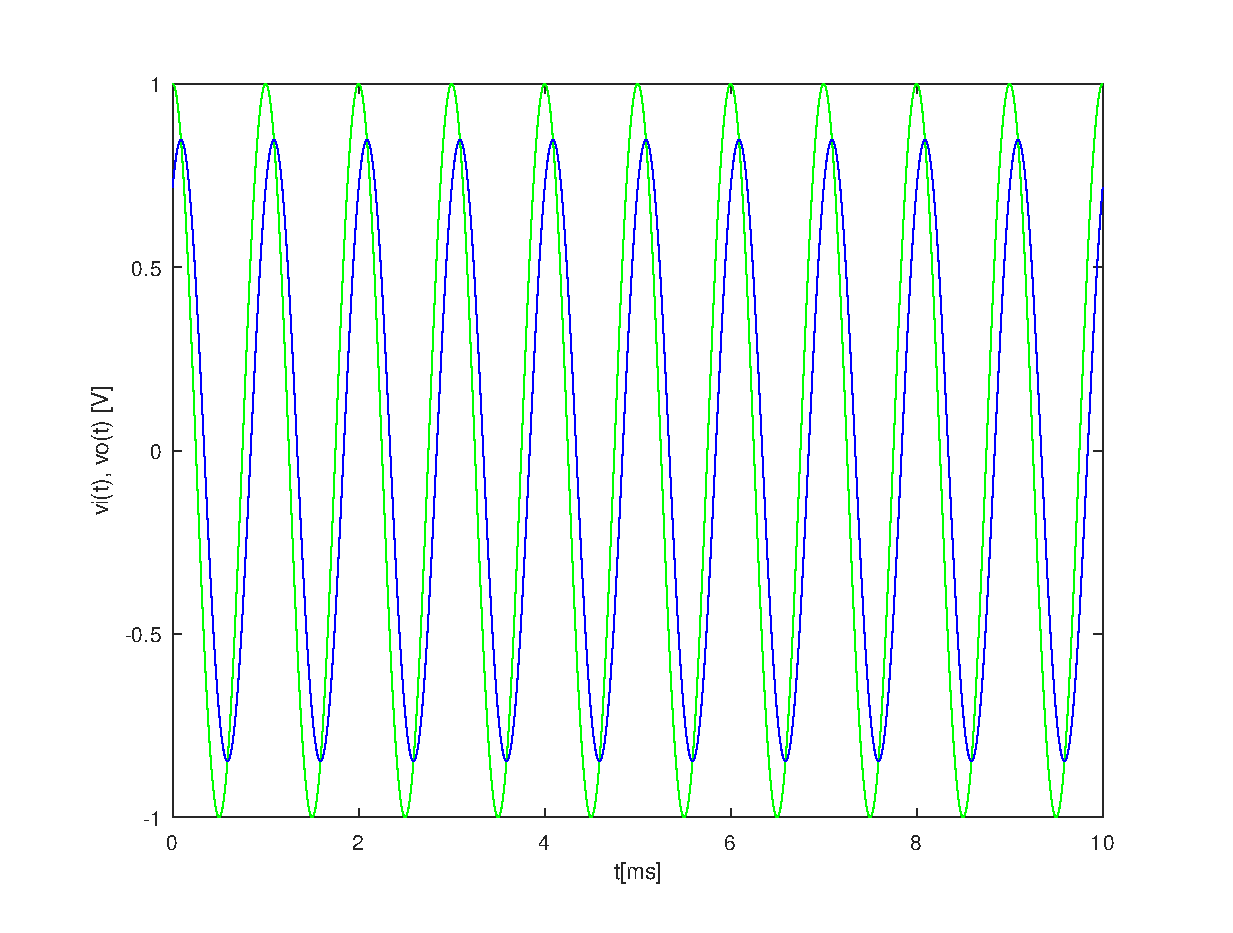
\includegraphics[width=0.8\linewidth]{forced.eps}
\caption{Forced sinusoidal response.}
\label{fig:forced}
\end{figure}





